\section{Usability Testing}
\subsection{การวางแผนการทดสอบ}
\begin{enumerate}
    % \item \textbf{Product under test}
    %       \begin{itemize}
    %         \item What's being tested?
    %         \item What are the business and experience goals of the product
    %       \end{itemize}
    \item \textbf{จุดประสงค์ของการทดสอบ}
          \begin{itemize}
              \item \textbf{เป้าหมายของการทดสอบ} : เพื่อวัดประสิทธิภาพการใช้งานของเว็บแอปพลิเคชันกับผู้ใช้
              \item \textbf{คำถามที่ใช้ในการทดสอบ} : เราได้เตรียมคำถามไว้ถามผู้ใช้หลังจากการทดสอบ โดยแบ่งคำถามออกเป็น 3 ประเภท \ref{tab:question-table} ดังนี้
                    \begin{table}[H]
                        \caption{ตารางคำถามที่ใช้ในการทดสอบ}
                        \label{tab:question-table}
                        \begin{tabularx}{\textwidth}{|l|>{\raggedright\arraybackslash}X|}
                            \cline{1-2}
                            \textbf{ประเภทคำถาม}                        & \textbf{คำถาม}                                                                  \\ \cline{1-2}
                            \multirow[t]{5}{*}{ความเหมาะสมของวิธีแก้ปัญหา} & Solution ที่เสนอแก้ปัญหาได้จริงไหม แก้ได้หมด หรือแก้ได้บางส่วน                             \\ \cline{2-2}
                                                                       & มีปัญหาหรือความต้องการอะไรอีกไหมที่ solution ยังไม่ตอบโจทย์                              \\ \cline{2-2}
                                                                       & ถ้าเทียบกับ solution อื่น ๆ ที่เคยใช้ คิดว่า solution นี้เป็นอย่างไร                         \\ \cline{2-2}
                                                                       & มีองค์ประกอบไหนที่ควรเติมเพื่อทำให้ solution มีประสิทธิภาพมากขึ้นในการ แก้ปัญหา                \\ \cline{2-2}
                                                                       & มีข้อจำกัดอะไรในการนำไปใช้งานจริงสำหรับกลุ่มเป้าหมาย เช่น ต้นทุน เวลา ความง่ายในการใช้งาน เป็นต้น \\ \cline{1-2}
                            \multirow[t]{4}{*}{การใช้งาน}               & Feature/function ไหนที่คิดว่าควรมี (แล้วยังไม่มี) หรือไม่จำเป็นต้องมี                         \\ \cline{2-2}
                                                                       & Feature/function ไหนที่คุณคิดว่ามีประโยชน์หรือไม่มีประโยชน์                               \\ \cline{2-2}
                                                                       & ลองให้คะแนนภาพรวมของ functions ของ solution นี้  1-10                             \\ \cline{2-2}
                                                                       & ทำยังไงให้ fuctions ของ solution ได้คะแนนเต็ม 10                                    \\ \cline{1-2}
                            \multirow[t]{5}{*}{ประสบการณ์ผู้ใช้}           & การใช้งาน solution ยาก/ง่ายอย่างไร เหมาะกับกลุ่มเป้าหมายไหม                           \\ \cline{2-2}
                                                                       & มีส่วนไหนของ solution ที่งงหรือใช้งานยาก                                             \\ \cline{2-2}
                                                                       & ชอบ solution/การใช้งานส่วนไหนมากที่สุด                                              \\ \cline{2-2}
                                                                       & ชอบ solution/การใช้งานส่วนไหนน้อยที่สุด                                              \\ \cline{2-2}
                                                                       & มีข้อเสนอแนะตรงไหนที่จะทำให้ประสบการณ์การใช้งาน solution ดีขึ้น                           \\ \cline{1-2}
                        \end{tabularx}
                    \end{table}
              \item \textbf{สมมติฐานที่ต้องการทดสอบ} : สมมติฐานที่ต้องการทดสอบคือเรื่องการใช้งานของทั้ง 3 ฟีเจอร์ ดังนี้
                    \begin{itemize}
                        \item Career Prediction : สามารถช่วยทำให้ผู้ใช้เห็นแนวทางของเรซูเมตัวเองมากขึ้นว่าเป็นอาชีพไหน
                        \item Career Insight : สามารถเห็นภาพรวมอาชีพและแนะนำการพัฒนาเรซูเมว่าควรมีทักษะอะไรเพิ่ม
                        \item Career Exploration : สามารถช่วยแนะนำทักษะที่ควรเรียนรู้ของสายอาชีพที่สนใจและอาชีพใกล้เคียง
                    \end{itemize}
          \end{itemize}
    \item \textbf{ผู้เข้าร่วมการทดสอบ}
          \begin{itemize}
              \item \textbf{จำนวนเข้าร่วมการทดสอบ} : 5 คน
              \item \textbf{ลักษณะสำคัญของกลุ่มเป้าหมายที่เข้าร่วมการทดสอบ} : นักศึกษาวิศวกรรมคอมพิวเตอร์ ที่สนใจจะทำอาชีพทางด้านเทคโนโลยีและมีความต้องการที่จะพัฒนาทักษะและเรซูเม
          \end{itemize}
    \item \textbf{ภารกิจที่มอบหมายให้ผู้เข้าร่วมทดสอบทำ} : ให้ผู้ทดสอบเริ่มทำนายสายอาชีพและดูข้อมูลของสายอาชีพที่ทำนายได้
\end{enumerate}
\subsection{การหาผู้เข้าร่วมการทดสอบ}
\begin{enumerate}
    \item \textbf{การคัดกรองผู้เข้าร่วมการทดสอบ}
          %   \begin{itemize}
          % \item คุณสมบัติที่ต้องมี (Include)
          \begin{table}[H]
              \caption{ตารางคุณสมบัติของผู้เข้าร่วมการทดสอบที่ต้องมี}
              \label{tab:my-table}
              \begin{tabularx}{\textwidth}{|X|X|X|}
                  \hline
                  \textbf{คุณสมบัติที่ต้องการ}             & \textbf{เกณฑ์การวัดคุณสมบัติ}                           & \textbf{คำถามที่ใช้สัมภาษณ์}   \\ \hline
                  นักศึกษาที่ข้อมูลเหมาะสมกับข้อมูลที่เรามี      & นักศึกษาวิศวกรรมคอมพิวเตอร์                             & คุณเรียนอยู่ภาควิชาอะไร       \\ \hline
                  ต้องการสมัครงาน                      & เรียนอยู่ปี 4, กำลังจะจบการศึกษา                          & ตอนนี้เรียนอยู่ชั้นปีอะไร        \\ \hline
                  ต้องการฝึกงาน                        & เรียนอยู่ปี 3, เรียนอยู่ปี 4, กำลังจะจบการศึกษา               & ตอนนี้เรียนอยู่ชั้นปีอะไร        \\ \hline
                  ต้องการค้นหาตนเอง                    & คนที่ไม่รู้ว่าตนเองอยากเป็นอาชีพอะไรกันแน่                   & สนใจทำอาชีพอะไรในอนาคต     \\ \hline
                  มีอาชีพที่อยากทำอยู่ในใจแล้ว               & คนที่มีอาชีพที่สนใจแต่อยากพัฒนาเรซูเมและทักษะให้ดีขึ้น           & มั่นใจในเรซูเมของตนเองแค่ไหน \\ \hline
                  กำลังสนใจอาชีพในสาย tech              & มีความสนใจในสายอาชีพ 6 อาชีพ ที่เรามีข้อมูล                & สนใจทำอาชีพอะไรในอนาคต     \\ \hline
                  ไม่มั่นใจว่าตนเองเหมาะสมกับอาชีพอะไรกันแน่ & รู้แล้วว่าตนเองชอบสายไหนแต่ยังไม่มั่นใจว่าจะทำอาชีพอะไรในสายนั้น & มั่นใจในอาชีพที่สนใจมากแค่ไหน  \\ \hline
                  ต้องการพัฒนาเรซูเม                    & คนที่มีเรซูเมอยู่แล้ว                                     & คุณมีเรซูเมหรือไม่            \\ \hline
              \end{tabularx}
          \end{table}
          % \item คุณสมบัติที่ไม่อยากได้ (Exclude)
          \begin{table}[H]
              \caption{ตารางคุณสมบัติของผู้เข้าร่วมการทดสอบที่ไม่อยากได้}
              \label{tab:excludeUT}
              \begin{tabularx}{\textwidth}{|X|X|X|}
                  \hline
                  \textbf{คุณสมบัติที่ไม่ต้องการ}      & \textbf{เกณฑ์การวัดคุณสมบัติ}             & \textbf{คำถามที่ใช้สัมภาษณ์}    \\ \hline
                  คนที่ยังไม่สนใจที่จะฝึกงานหรือสมัครงาน & คนที่ยังศึกษาไม่ถึงระดับปริญญาตรี             & โปรดระบุระดับการศึกษาของคุณ   \\ \hline
                  ไม่ได้สนใจงานทางด้านสาย tech     & คนที่สนใจสายงานอื่นนอกจาก 6 สายที่เรามีข้อมูล & คุณสนใจทำสายอาชีพอะไรในอนาคต \\ \hline
              \end{tabularx}
          \end{table}
          %   \end{itemize}
    \item \textbf{การนัดหมายผู้เข้าร่วมการทดสอบ}
          \begin{table}[H]
              \caption{ตารางนัดหมายการทดสอบ}
              \label{tab:schedule-UT}
              \begin{tabular}{|r|l|l|l|l|}
                  \hline
                  \multicolumn{1}{|l|}{\textbf{วันที่}} & \textbf{เวลานัดหมาย} & \textbf{กำหนดการ}   & \textbf{ผู้สัมภาษณ์} & \textbf{ผู้จดข้อมูล}            \\ \hline
                  \multirow[t]{5}{*}{16/03/2024}     & 16:30-17:00         & ผู้เข้าร่วมทดสอบ คนที่ 1 & นริศ ถนอมทรัพย์     & ณิวัฒน์ชัย หวังตระกูลดี            \\ \cline{2-5}
                                                     & 17:00-17:30         & ผู้เข้าร่วมทดสอบ คนที่ 2 & นริศ ถนอมทรัพย์     & ณิวัฒน์ชัย หวังตระกูลดี            \\ \cline{2-5}
                                                     & 17:30-20:30         & พัก                 & -                & -                           \\ \cline{2-5}
                                                     & 20:30-21:00         & ผู้เข้าร่วมทดสอบ คนที่ 3 & นริศ ถนอมทรัพย์     & ณิวัฒน์ชัย หวังตระกูลดี            \\ \cline{2-5}
                                                     & 21:00-22:00         & ผู้เข้าร่วมทดสอบ คนที่ 4 & นริศ ถนอมทรัพย์     & นภัทร วารีดี                   \\ \hline
                  \multirow[t]{2}{*}{17/03/2024}     & 14:30-15:00         & ผู้เข้าร่วมทดสอบ คนที่ 5 & นริศ ถนอมทรัพย์     & นภัทร วารีดี, ณิวัฒน์ชัย หวังตระกูลดี \\ \cline{2-5}
                                                     & 15:00-16:00         & สรุปผล              & -                & -                           \\ \hline
              \end{tabular}
          \end{table}
\end{enumerate}
\subsection{การเตรียมการทดสอบ}
\begin{enumerate}
    \item \textbf{Prototype} : \href{https://compath-cpe.web.app/}{Compath-MVP (Production Server)}
    \item \textbf{แพลตฟอร์มสำหรับการทดสอบ} : Discord
    \item \textbf{แพลตฟอร์มสำหรับจดบันทึก} : FigJam
    \item \textbf{สถานการณ์และภารกิจ}
          \begin{table}[H]
              \caption{ตารางสถานการณ์และภารกิจที่มอบหมายให้ผู้เข้าร่วมทดสอบ}
              \label{tab:scenarioUT}
              \begin{tabularx}{\textwidth}{|l|X|}
                  \hline
                  \textbf{Scenario 1} & \textbf{คุณต้องการรู้ว่าเรซูเมของคุณเหมาะกับอาชีพที่คุณอยากเป็นหรือยัง รวมถึงอยากรู้ว่าต้องพัฒนาตัวเองอย่างไร} \\ \hline
                  Task 1              & เริ่มทำนายสายอาชีพ                                                                          \\ \hline
                  Success path        & ทำนายสายอาชีพสำเร็จ ได้ผลลัพธ์ออกมาเป็นสายอาชีพ                                                  \\ \hline
                  Task 2              & ดูข้อมูลเชิงลึกของอาชีพที่ทำนายได้                                                                \\ \hline
                  Success path        & ดูทักษะที่จำเป็นในการเป็นอาชีพที่สนใจ                                                             \\ \hline
                  Task 3              & ดูอาชีพใกล้เคียงของอาชีพที่ตอนเองสนใจ                                                          \\ \hline
                  Success path        & เข้ามาดูหน้าสายใยอาชีพพร้อมกับลองกดดูทักษะของอาชีพอื่น ๆ                                           \\ \hline
              \end{tabularx}
          \end{table}
    \item \textbf{บทพูดสำหรับการดำเนินการทดสอบ}
          \begin{figure}[H]\centering
              \fbox{
\includegraphics[width=14cm]{./figure/UT/ScriptUT.png}}
              \caption{รูปแสดงบทพูดสำหรับการดำเนินการทดสอบ}\label{fig:ScriptUT}
          \end{figure}
    \item \textbf{การวัดผลเชิงปริมาณ} การวัดผลเชิงปริมาณมีผู้เข้าร่วมการประเมินทั้งหมด 70 คน แบ่งเป็นแต่ละชั้นปี ดังรูป \ref{fig:UserRatio}  โดยผู้เข้ารวมการประเมินได้ทดลองใช้งานเว็บแอปพลิเคชันและทำ\href{https://forms.office.com/r/CRHVxtCC4t}{แบบสอบถามเพื่อวัดผลเชิงปริมาณ}
          \begin{figure}[H]\centering
              \fbox{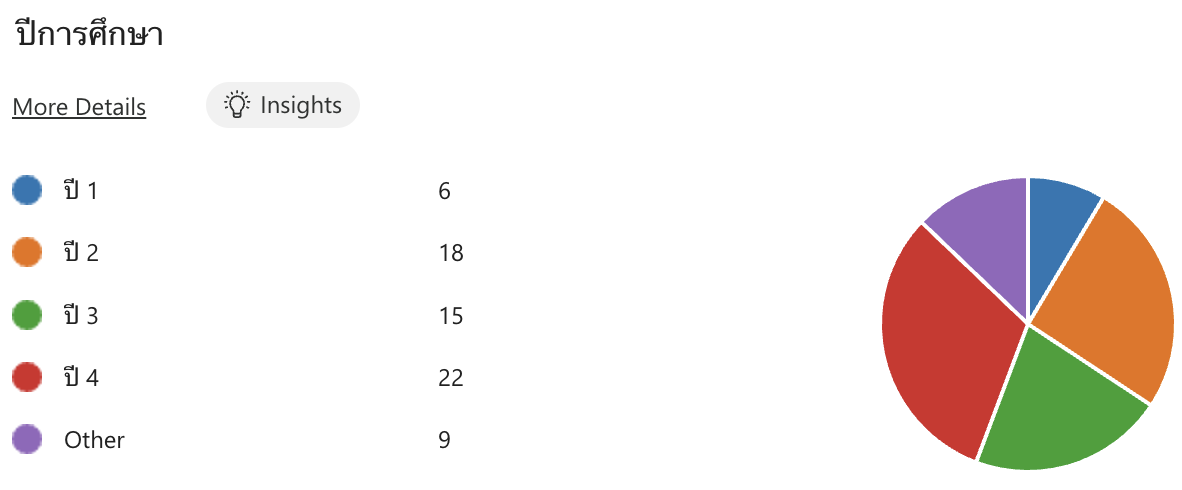
\includegraphics[width=14cm]{./figure/UT/UserRatio.png}}
              \caption{รูปแสดงจำนวนและอัตราส่วนผู้เข้าร่วมการประเมิน}\label{fig:UserRatio}
          \end{figure}
          \begin{table}[H]
              \caption{ตารางแสดงจำนวนและอัตราส่วนของผู้เข้าร่วมการประเมิน}
              \label{tab:UserRatio}
              \begin{tabular}{|l|r|r|}
                  \hline
                  \textbf{ปีการศึกษา} & \multicolumn{1}{l|}{\textbf{จำนวนผู้เข้าร่วมการประเมิน}} & \multicolumn{1}{l|}{\textbf{อัตราส่วนร้อยละ}} \\ \hline
                  ปี 1               & 6                                                  & 8.57\%                                     \\ \hline
                  ปี 2               & 18                                                 & 25.71\%                                    \\ \hline
                  ปี 3               & 15                                                 & 21.43\%                                    \\ \hline
                  ปี 4               & 22                                                 & 31.43\%                                    \\ \hline
                  อื่น ๆ              & 9                                                  & 12.86\%                                    \\ \hline
              \end{tabular}
          \end{table}
          \par{ซึ่งได้ผลลัพท์การประเมินออกมาดังภาพ \ref{fig:QuantitativeResult} โดยมีเกณฑ์การประเมิน คือ [1 - ไม่เห็นด้วยอย่างยิ่ง, 5 - เห็นด้วยอย่างยิ่ง]}
          \begin{figure}[H]\centering
              \fbox{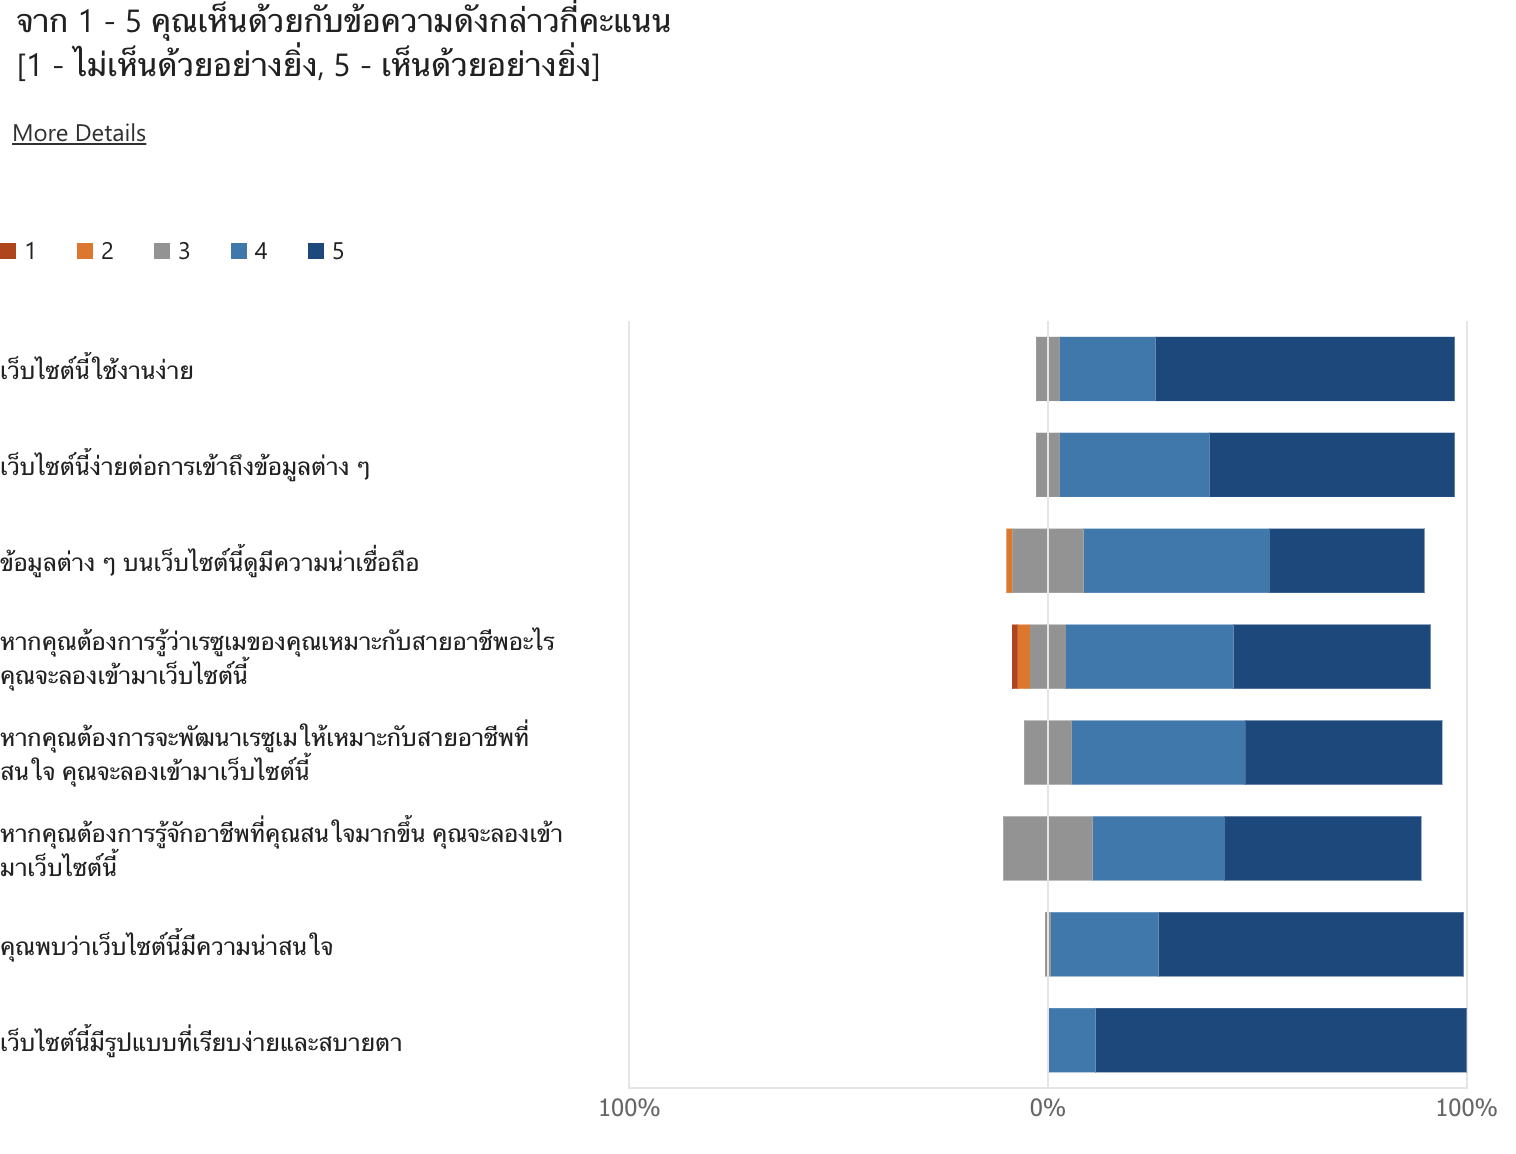
\includegraphics[width=14cm]{./figure/UT/QuantitativeResult.png}}
              \caption{รูปแสดงผลลัพธ์การประเมินเว็บแอปพลิเคชัน Compath}\label{fig:QuantitativeResult}
          \end{figure}
          โดยนำคะแนนในแต่ละหัวข้อการประเมินมาเฉลี่ย โดยมีคะแนนเต็มอยู่ที่ 5 ดังตาราง ได้ดังนี้
          \begin{table}[H]
              \caption{ตารางแสดงผลลัพธ์การประเมินเว็บแอปพลิเคชัน Compath}
              \label{tab:QuantitativeResult}
              \begin{tabular}{|l|rrrrr|r|}
                  \hline
                  \multicolumn{1}{|c|}{\multirow{2}{*}{\textbf{หัวข้อการประเมิน}}}                                              & \multicolumn{5}{c|}{\textbf{อัตราส่วนการให้คะแนน}} & \multicolumn{1}{c|}{\multirow{2}{*}{\textbf{คะแนนเฉลี่ย}}}                                                                                                                               \\ \cline{2-6}
                  \multicolumn{1}{|c|}{}                                                                                     & \multicolumn{1}{c|}{\textbf{1}}                 & \multicolumn{1}{c|}{\textbf{2}}                          & \multicolumn{1}{c|}{\textbf{3}} & \multicolumn{1}{c|}{\textbf{4}} & \multicolumn{1}{c|}{\textbf{5}} & \multicolumn{1}{c|}{} \\ \hline
                  เว็บไซต์นี้ใช้งานง่าย                                                                                            & \multicolumn{1}{r|}{0\%}                        & \multicolumn{1}{r|}{0\%}                                 & \multicolumn{1}{r|}{5.7\%}      & \multicolumn{1}{r|}{22.9\%}     & 71.4\%                          & 4.66                  \\ \hline
                  เว็บไซต์นี้ง่ายต่อการเข้าถึงข้อมูลต่าง ๆ                                                                              & \multicolumn{1}{r|}{0\%}                        & \multicolumn{1}{r|}{0\%}                                 & \multicolumn{1}{r|}{5.7\%}      & \multicolumn{1}{r|}{35.7\%}     & 58.6\%                          & 4.51                  \\ \hline
                  ข้อมูลต่าง ๆ บนเว็บไซต์นี้ดูมีความน่าเชื่อถือ                                                                           & \multicolumn{1}{r|}{0\%}                        & \multicolumn{1}{r|}{1.4\%}                               & \multicolumn{1}{r|}{17.1\%}     & \multicolumn{1}{r|}{44.3\%}     & 37.1\%                          & 4.18                  \\ \hline
                  \begin{tabular}[c]{@{}l@{}}หากคุณต้องการรู้ว่าเรซูเมของคุณเหมาะกับสายอาชีพอะไร\\  คุณจะลองเข้ามาเว็บไซต์นี้\end{tabular}  & \multicolumn{1}{r|}{1.4\%}                      & \multicolumn{1}{r|}{2.9\%}                               & \multicolumn{1}{r|}{8.6\%}      & \multicolumn{1}{r|}{40\%}       & 47.1\%                          & 4.26                  \\ \hline
                  \begin{tabular}[c]{@{}l@{}}หากคุณต้องการจะพัฒนาเรซูเมให้เหมาะกับสายอาชีพที่สนใจ \\ คุณจะลองเข้ามาเว็บไซต์นี้\end{tabular} & \multicolumn{1}{r|}{0\%}                        & \multicolumn{1}{r|}{0\%}                                 & \multicolumn{1}{r|}{11.4\%}     & \multicolumn{1}{r|}{41.4\%}     & 47.1\%                          & 4.34                  \\ \hline
                  \begin{tabular}[c]{@{}l@{}}หากคุณต้องการรู้จักอาชีพที่คุณสนใจมากขึ้น \\ คุณจะลองเข้ามาเว็บไซต์นี้\end{tabular}              & \multicolumn{1}{r|}{0\%}                        & \multicolumn{1}{r|}{0\%}                                 & \multicolumn{1}{r|}{21.4\%}     & \multicolumn{1}{r|}{31.4\%}     & 47.1\%                          & 4.24                  \\ \hline
                  คุณพบว่าเว็บไซต์นี้มีความน่าสนใจ                                                                                   & \multicolumn{1}{r|}{0\%}                        & \multicolumn{1}{r|}{0\%}                                 & \multicolumn{1}{r|}{1.4\%}      & \multicolumn{1}{r|}{25.7\%}     & 72.9\%                          & 4.71                  \\ \hline
                  เว็บไซต์นี้มีรูปแบบที่เรียบง่ายและสบายตา                                                                             & \multicolumn{1}{r|}{0\%}                        & \multicolumn{1}{r|}{0\%}                                 & \multicolumn{1}{r|}{0\%}        & \multicolumn{1}{r|}{11.4\%}     & 88.6\%                          & 4.88                  \\ \hline
                  \multicolumn{6}{|l|}{\textbf{คะแนนเฉลี่ยรวม}}                                                                & \textbf{4.47}                                                                                                                                                                                                                            \\ \hline
              \end{tabular}
          \end{table}

          จากผลลัพธ์ดังกล่าว จะเห็นได้ว่า เว็บแอปพลิเคชันได้รับผลตอบรับที่ดี มีแนวโน้มในเชิงบวก และได้รับคะแนนเฉลี่ยอยู่ที่ 4.47 คะแนนจาก 5 ซึ่งนับเป็น 89\%
          นับว่าประสบความสำเร็จตามเป้าหมายที่วางเอาไว้

\end{enumerate}
\subsection{การดำเนินการทดสอบ}
\begin{enumerate}
    \item \textbf{ข้อกำหนดในการทดสอบ}
          \begin{enumerate}
              \item \textbf{กระตุ้นให้ผู้ร่วมทดสอบพูดในสิ่งที่กำลังคิดอยู่} เพื่อให้สามารถสังเกตความเข้าใจในการใช้งานของผู้เข้าร่วมการทดสอบได้มากขึ้น
              \item \textbf{ไม่ชี้นำระหว่างทำการทดสอบ} เพื่อให้การทดสอบเปรียบเสมือนการใช้งานจริงมากที่สุด
              \item \textbf{ไม่อธิบายการใช้งาน} เพื่อทดสอบการใช้งานของผู้ใช้โดยไม่มีการสอนวิธีการใช้มาก่อน
          \end{enumerate}
    \item \textbf{การจดบันทึกระหว่างการทดสอบ} โดยหลังจากที่ผู้ทดสอบทำการใช้งานเว็บแอปพลิเคชันเรียบร้อยแล้ว จะมีการถามคำถามเพื่อเก็บข้อมูลเพิ่มเติมจากผู้ใช้และจดบันทึกเพื่อนำไปวิเคราะห์ปัญหาที่เกิดขึ้นระหว่างการใช้งานเว็บแอปพลิเคชัน ดังรูป \ref{fig:NoteTaking}
          \begin{figure}[H]\centering
              \fbox{\includegraphics[width=14cm]{./figure/UT/NoteTaking.png}}
              \caption{รูปแสดงการจดบันทึกระหว่างการทดสอบ}\label{fig:NoteTaking}
          \end{figure}
\end{enumerate}
\subsection{วิเคราะห์ผลการทดสอบ}
\begin{enumerate}
    \item \textbf{เก็บรวมรวมปัญหาระหว่างการทดสอบ} โดยแบ่งปัญหาออกเป็นของแต่ละฟีเจอร์เพื่อให้ง่ายต่อการแยกประเภทของปัญหา ดังรูป \ref{fig:GateringIssue}
          \begin{figure}[H]\centering
              \fbox{\includegraphics[width=14cm]{./figure/UT/GateringIssue.png}}
              \caption{รูปแสดงการจดบันทึกปัญหาที่พบ}\label{fig:GateringIssue}
          \end{figure}
          \begin{figure}[H]\centering
              \fbox{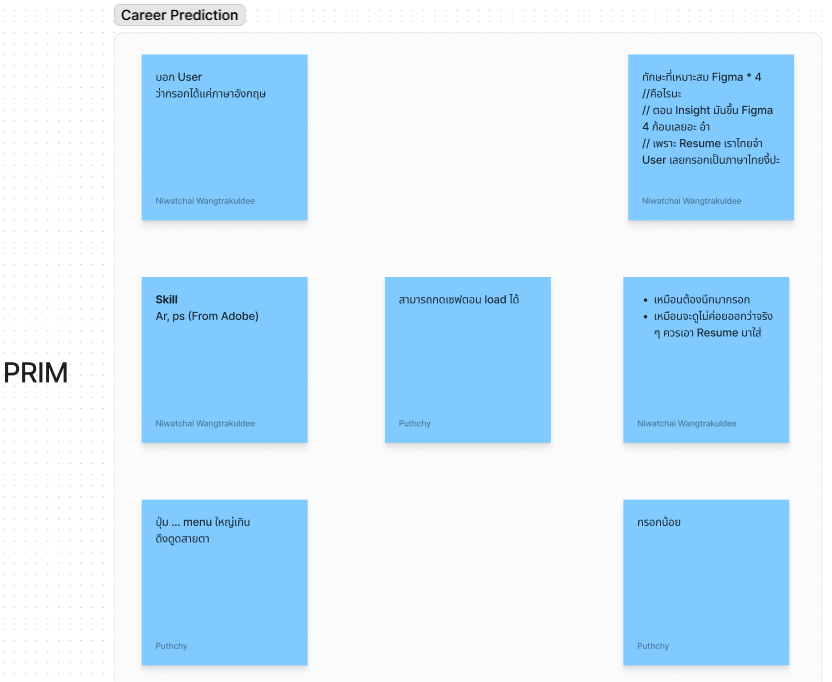
\includegraphics[width=14cm]{./figure/UT/exam-GateringIssue.png}}
              \caption{รูปแสดงตัวอย่างปัญหาที่พบ}\label{fig:exam-GateringIssue}
          \end{figure}
    \item \textbf{จัดประเภทของปัญหา} โดยจะจัดประเภทของปัญหาที่เกิดขึ้นระหว่างการทำแบบทดสอบเพื่อให้สามารถเห็นความถี่ของปัญหาที่เกิดขึ้นได้ง่ายมากยิ่งขึ้น ดังรูป \ref{fig:Groping}
          \begin{figure}[H]\centering
              \fbox{\includegraphics[width=14cm]{./figure/UT/Groping.png}}
              \caption{รูปแสดงการจัดประเภทของปัญหา}\label{fig:Groping}
          \end{figure}
          \begin{figure}[H]\centering
              \fbox{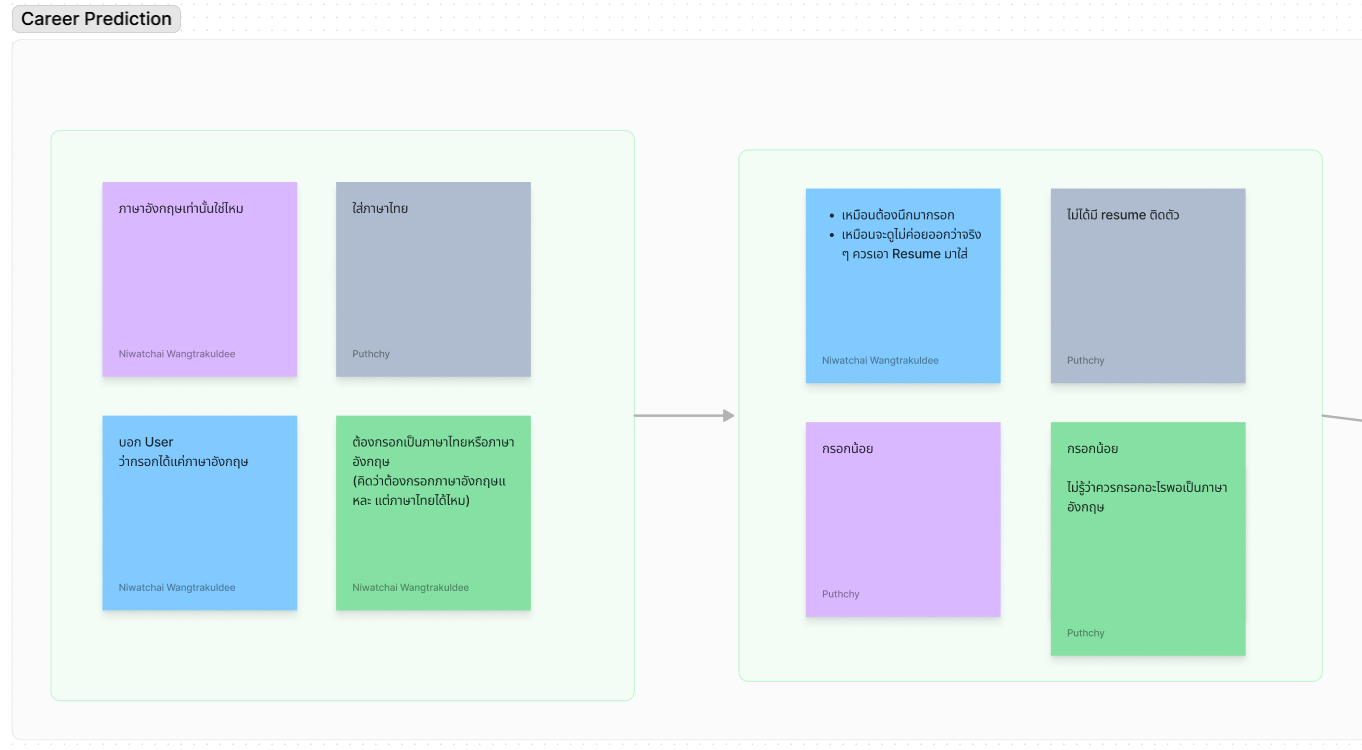
\includegraphics[width=14cm]{./figure/UT/exam-Groping.png}}
              \caption{รูปแสดงตัวอย่างการจัดประเภทของปัญหา}\label{fig:exam-Groping}
          \end{figure}
    \item \textbf{นิยามประเภทของปัญหา} โดยจะนิยามประเภทของปัญหาเพื่อให้สามารถเข้าใจปัญหาที่เกิดขึ้นและสามารถคิดวิธีแก้ปัญหาออกมาได้ ดังรูป \ref{fig:CreateTheme}
          \begin{figure}[H]\centering
              \fbox{\includegraphics[width=14cm]{./figure/UT/CreateTheme.png}}
              \caption{รูปแสดงการนิยามประเภทของปัญหา}\label{fig:CreateTheme}
          \end{figure}
          \begin{figure}[H]\centering
              \fbox{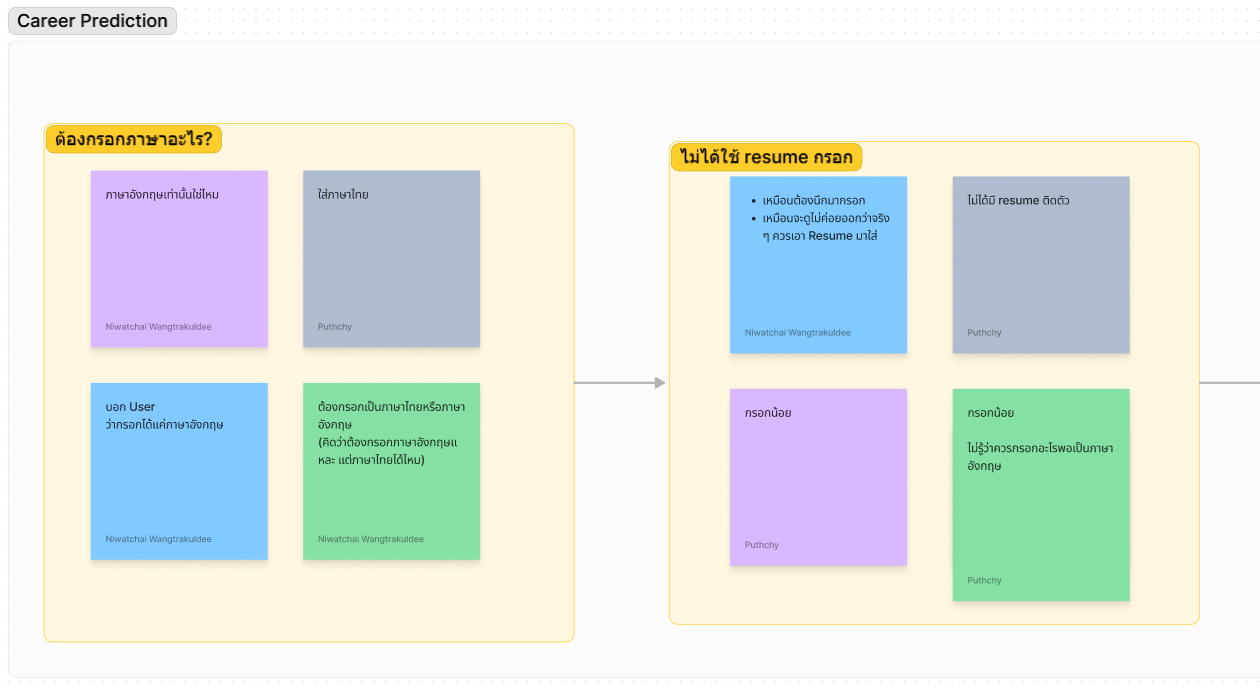
\includegraphics[width=14cm]{./figure/UT/exam-CreateTheme.png}}
              \caption{รูปแสดงตัวอย่างการนิยามประเภทของปัญหา}\label{fig:exam-CreateTheme}
          \end{figure}
          \begin{enumerate}
              \item \textbf{Career Prediction}
                    \begin{itemize}
                        \item ไม่มั่นใจว่าต้องกรอกข้อมูลเป็นภาษาอะไร
                        \item ไม่ได้ใช้เรซูเมในการกรอก
                        \item ไม่มั่นใจในการกรอกข้อมูลส่วนต่าง ๆ
                        \item กรอกสิ่งที่คาดไม่ถึง
                        \item กดปุ่มระหว่างรอผลทำนาย
                        \item สับสนตอนดูผลทำนาย
                    \end{itemize}
              \item \textbf{Career Insight}
                    \begin{itemize}
                        \item ไม่ทราบว่าสามารถดูประวัติการทำนายอื่น ๆ ได้จากอาชีพนี้
                        \item พบปัญหาการใช้ส่วนที่แสดงทักษะ
                        \item สับสนการแสดงกราฟและทักษะ
                        \item ไม่ได้กดเข้าไปดูสายใยอาชีพต่อ
                    \end{itemize}
              \item \textbf{Career Exploration}
                    \begin{itemize}
                        \item ไม่ทราบว่าสามารถกดเพื่อดูทักษะของอาชีพที่แสดงอยู่ได้
                        \item หมวดหมู่ของทักษะแสดงทับกัน
                    \end{itemize}
          \end{enumerate}
    \item \textbf{ลำดับความสำคัญของปัญหาพี่พบ} โดยจะจัดลำดับความสำคัญของปัญหาที่เกิดขึ้นจาก 2 ปัจจัย คือ ความสำคัญของปัญหา และความถี่ที่เกิดขึ้นของปัญหา ดังรูป \ref{fig:PrioritizeUT}
          \begin{figure}[H]\centering
              \fbox{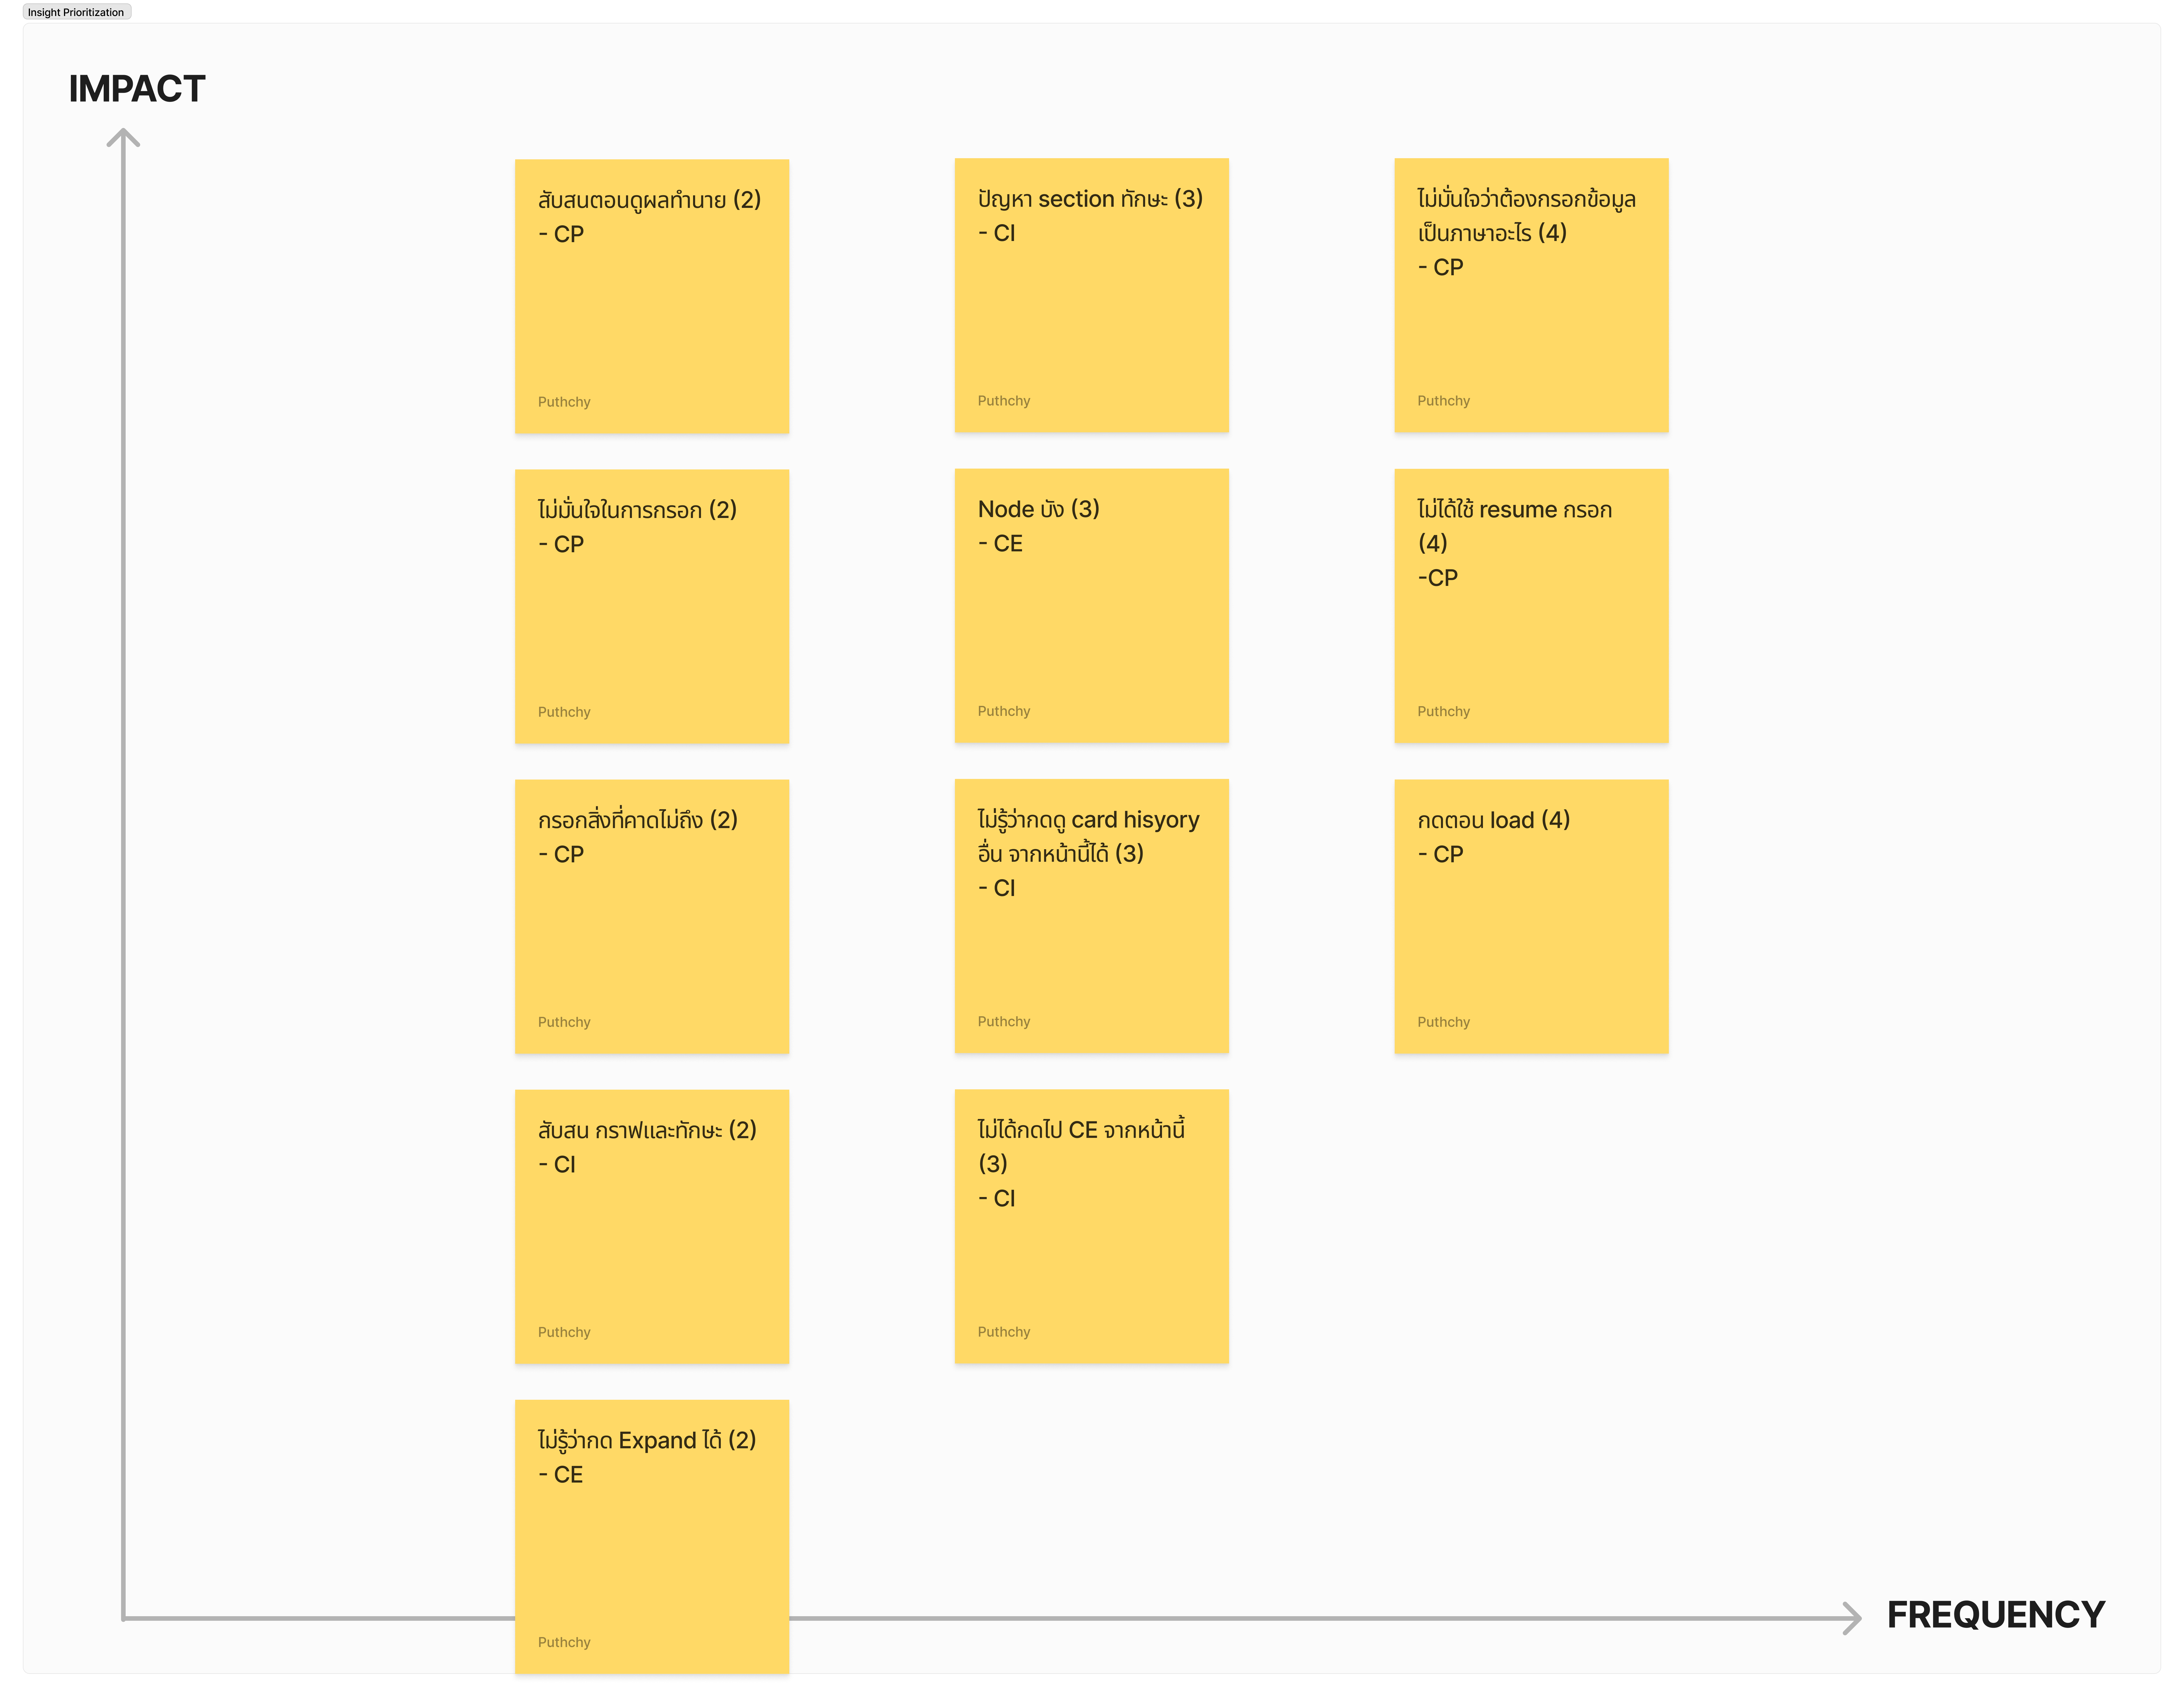
\includegraphics[width=14cm]{./figure/UT/PrioritizeUT.png}}
              \caption{รูปแสดงการเรียงลำดับความสำคัญของปัญหาพี่พบ}\label{fig:PrioritizeUT}
          \end{figure}
    \item \textbf{คำแนะนำสำหรับปัญหาที่พบ} โดยการแนะนำแนวทางการแก้ไขปัญหาที่พบและระบุความยากของการแก้ไขปัญหา ดังตาราง \ref{tab:recommendationsUT}
          \begin{table}[H]
              \caption{แนะนำแนวทางวิธีการแก้ไขปัญหา}
              \label{tab:recommendationsUT}
              \begin{tabularx}{\textwidth}{|l|>{\raggedright\arraybackslash}X|l|>{\raggedright\arraybackslash}X|>{\raggedright\arraybackslash}X|}
                  \hline
                  \textbf{ประเภทของปัญหา}             & \textbf{ปัญหาที่พบ}                    & \textbf{หน้า}       & \textbf{แนวทางการแก้ไขปัญหา}                          & \textbf{ระดับความยากในการแก้ไขปัญหา} \\ \hline
                  \multirow[t]{2}{*}{คำชี้แจงไม่ชัดเจน}   & ไม่มั่นใจว่าต้องกรอกข้อมูลเป็นภาษาอะไร      & Career Prediction  & มีข้อความระบุให้กรอกข้อมูลเป็นภาษาอังกฤษ                    & ปานกลาง                           \\ \cline{2-5}
                                                     & ไม่ได้ใช้เรซูเมกรอก                     & Career Prediction  & แบ่ง section การกรอกให้ละเอียดมากขึ้น                    & ยาก                               \\ \hline
                  ปุ่มสามารถกดได้ระหว่างโหลด             & กดตอนโหลด                           & Career Prediction  & ปิดการใช้งานปุ่มระหว่างการรอโหลด                         & ง่าย                               \\ \hline
                  String Matching                    & ปัญหาในส่วนทักษะ                       & Career Insight     & นำเทคนิคการตรวจจับคำที่ดีขึ้นมาใช้                            & ยาก                               \\ \hline
                  Technical Issue                    & หมวดหมู่ของทักษะแสดงทับกัน               & Career Exploration & ทำ Auto Layout ให้กับผังหมวดหมู่ของทักษะ                   & ปานกลาง                           \\ \hline
                  \multirow[t]{3}{*}{User Interface} & ไม่รู้ว่ากดดูการทำนายอื่น ๆ จากหน้านี้ได้       & Career Insight     & ย้ายส่วนของการเลือกประวัติการทำนายมาไว้ในส่วนที่มองเห็นง่ายกว่านี้ & ปานกลาง                           \\ \cline{2-5}
                                                     & ไม่ได้กดไป Career Exploration จากหน้านี้ & Career Insight     & ทำส่วนที่แนะนำให้ไปดูสายใยอาชีพให้ดึงดูมากกว่านี้                 & ปานกลาง                           \\ \cline{2-5}
                                                     & สับสนตอนดูผลทำนาย                      & Career Prediction  & ลดจำนวนปุ่ม, ทำเป็นบันทึกอัตโนมัติ                            & ปานกลาง                           \\ \hline
                  คำชี้แจงไม่ชัดเจน                       & ไม่มั่นใจในการกรอก                     & Career Prediction  & ยกตัวอย่างทักษะให้มากและชัดเจนมากกว่านี้                    & ปานกลาง                           \\ \hline
                  Machine Learning Limitation        & กรอกสิ่งที่คาดไม่ถึง                      & Career Prediction  & เทรนข้อมูลเพิ่ม                                         & ยาก                               \\ \hline
                  \multirow[t]{2}{*}{User Interface} & สับสน กราฟและทักษะ                    & Career Insight     & เขียนอธิบายกราฟว่าเชื่องโยงกับทักษะอย่างไร                  & ปานกลาง                           \\ \cline{2-5}
                                                     & ไม่รู้ว่ากด Expand ได้                   & Career Exploration & สร้าง tooltips สำหรับการใช้งาน                          & ปานกลาง                           \\ \hline
              \end{tabularx}
          \end{table}
    \item \textbf{ลำดับความสำคัญของคำแนะนำ} โดยจะเรียงลำดับคำแนะนำแนวทางการแก้ไขปัญหาจาก 2 ปัจจัย คือ เป็นประโยชน์กับผู้ใช้งานและความยากในการแก้ไขปัญหา ดังรูป \ref{fig:PriRec}
          \begin{figure}[H]\centering
              \fbox{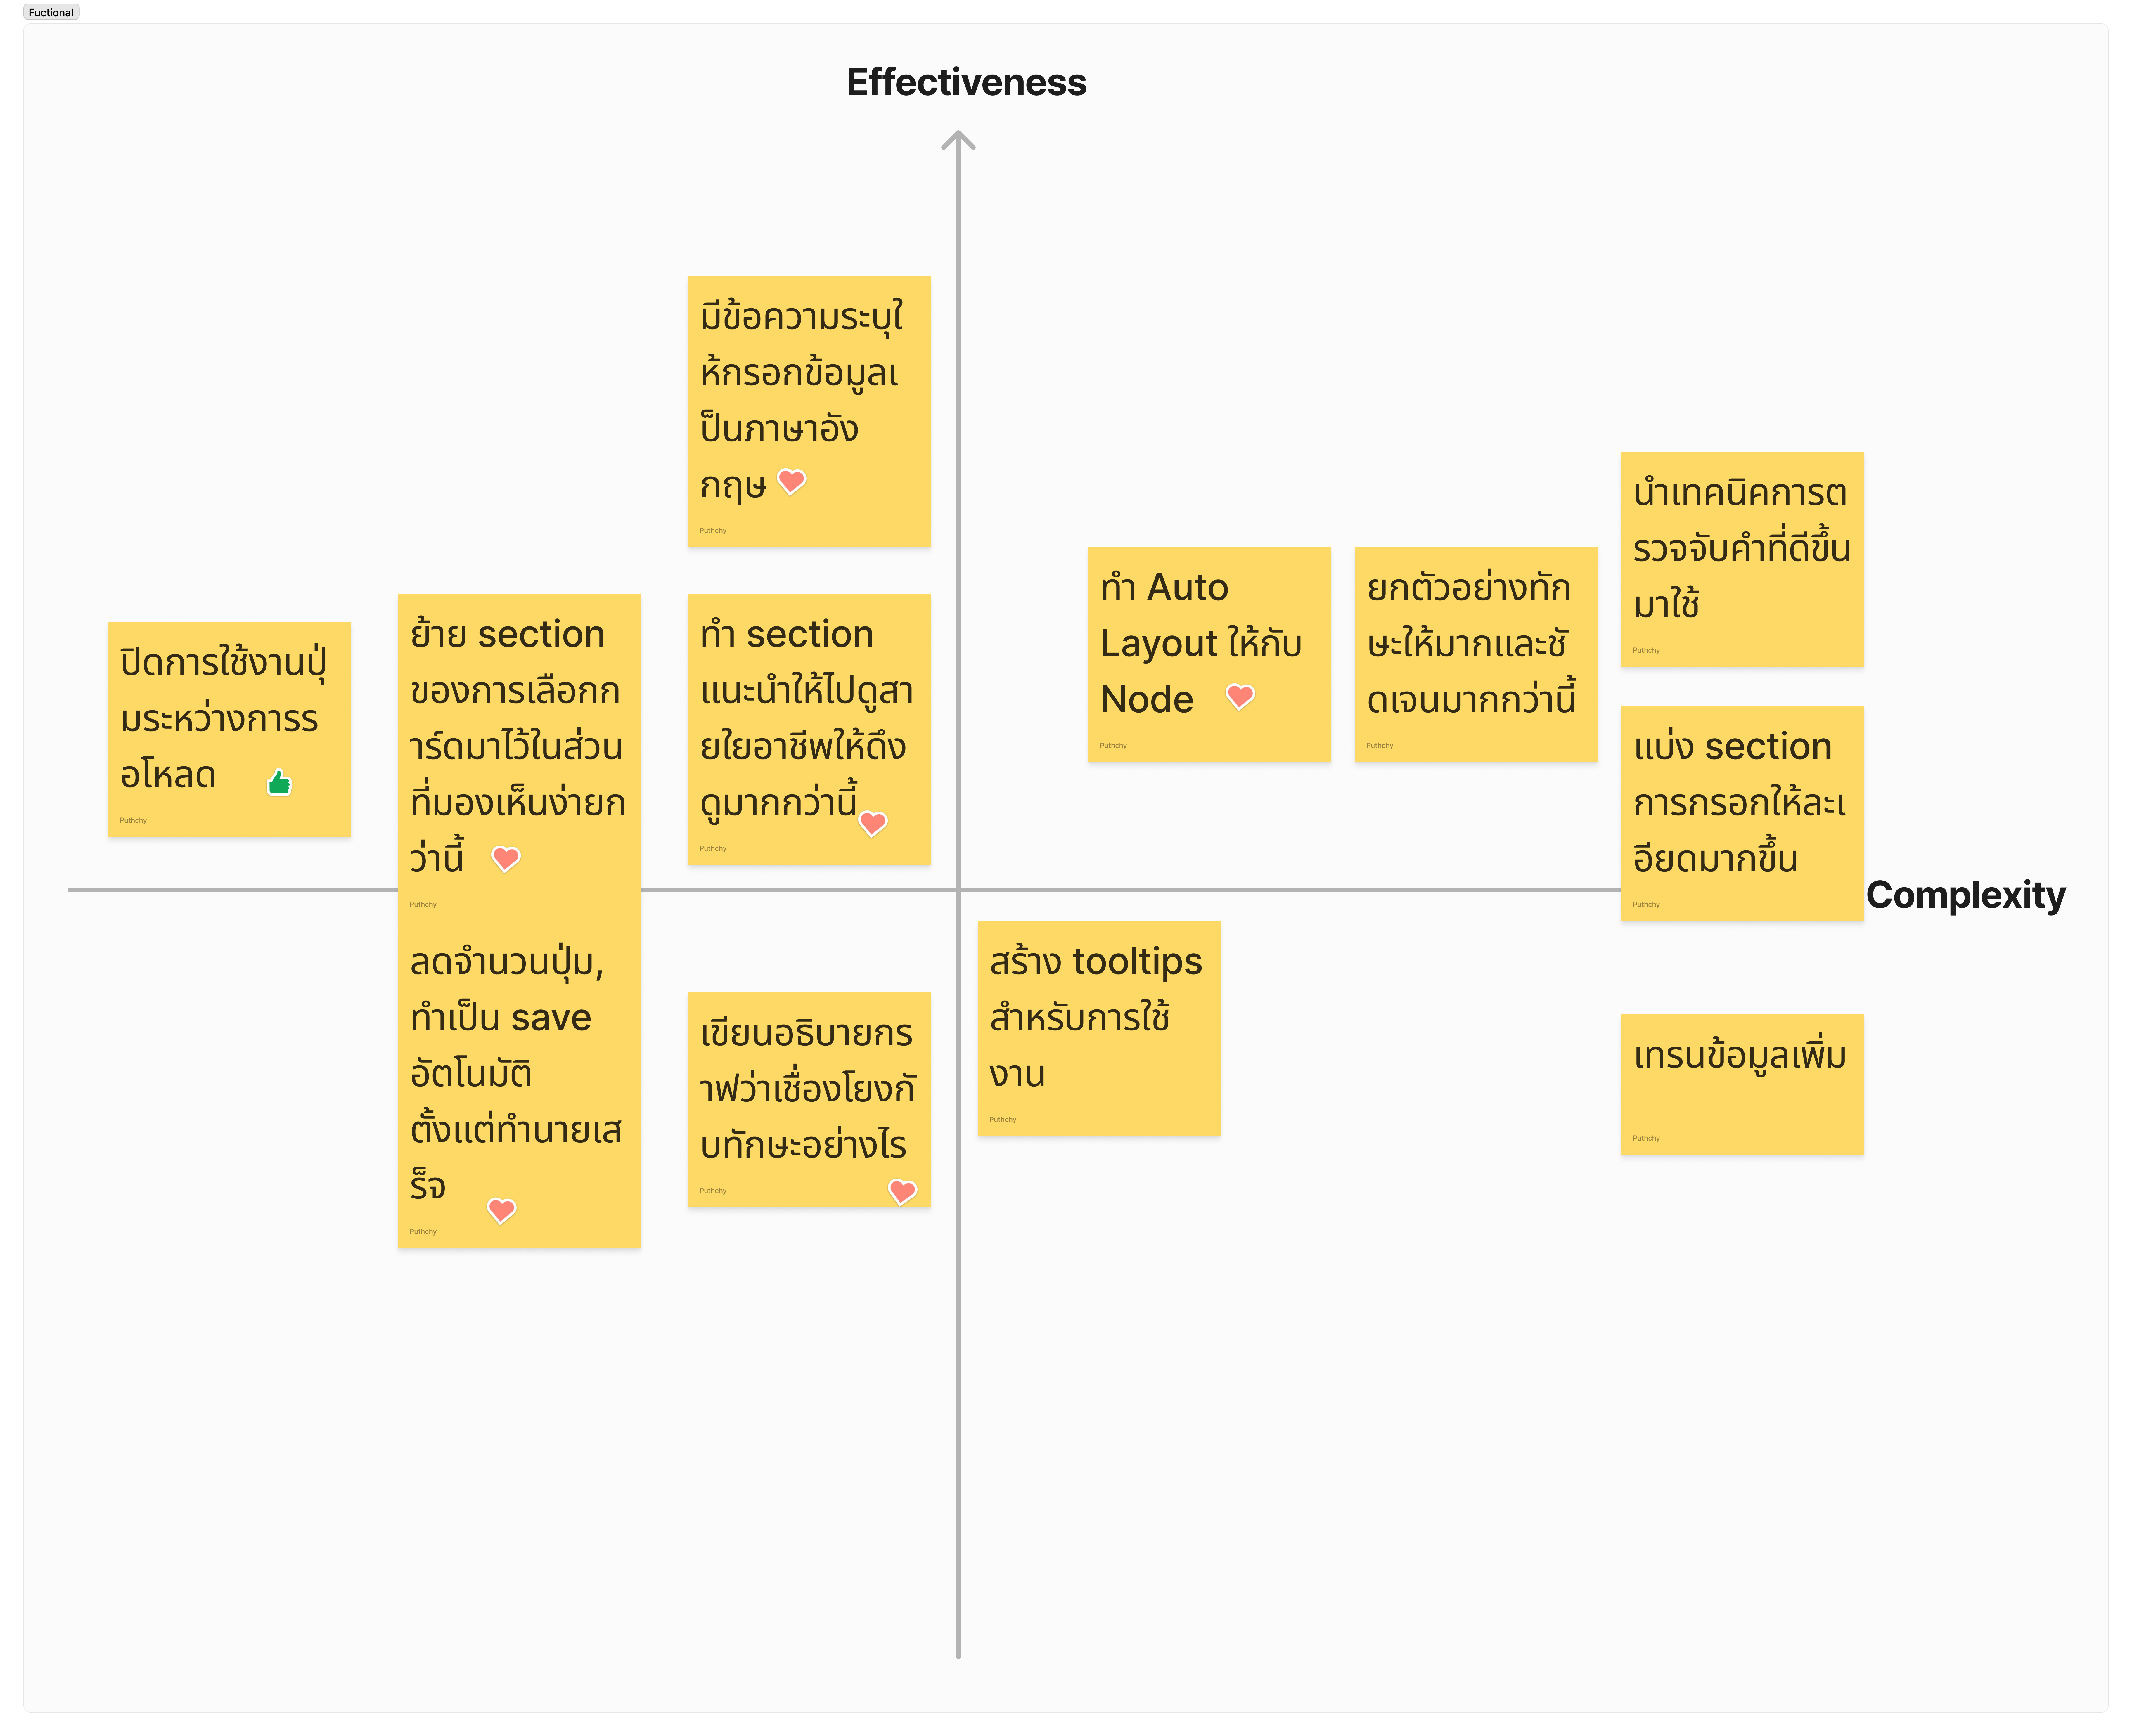
\includegraphics[width=14cm]{./figure/UT/PriRec.png}}
              \caption{รูปแสดงการเรียงลำดับความสำคัญของปัญหาพี่พบ}\label{fig:PriRec}
          \end{figure}
\end{enumerate}
